\subsection{E9 --- Objection 4: should placement differ for reusable, streamed and randomly accessed data?}
\label{sec:e9}
\textbf{Question.} The same system may process a highly reusable dataset, a streaming dataset and a randomly accessed one. Everything up to E8 read each entry every step, so reuse was uniform. Does the best placement depend on the access regime, and can the runtime adapt without being told the regime? \textbf{Setup.} The three regimes of Sec.~\ref{sec:sys} (reusable = dense; random with 30\%, 10\% and 3\% of entries read per step; streaming = each entry read once), 42 traces, 16 CIM units, in-memory compute. Policies: static modality, the dynamic policy ($8\times/0.4\times$, not re-tuned for any regime) and the reuse-aware policy of Sec.~\ref{sec:sys}, each at the bottom-up migration cost and at $10\times$ that cost (a stress setting, equal to the cost assumed in E1--E7). Random draws use one seed per trace, so every policy sees the same reads. H9a--H9e were written down after the runs were launched and before any result was inspected.

\begin{table}[t]
\centering\small
\caption{E9: change against static modality (mean over 42 traces; energy and quality loss in \%, negative is better). ``Gate'' is the reuse-aware policy (the post-hoc variant of Sec.~\ref{sec:e9} is in Fig.~\ref{fig:e9}). Flat/static is the energy headroom of \warm{} in that regime.}
\label{tab:e9}
\setlength{\tabcolsep}{4pt}
\begin{tabular}{lcccccccc}
\toprule
 & Flat/ & \multicolumn{3}{c}{Dynamic, bottom-up cost} & \multicolumn{2}{c}{Dynamic, $10\times$} & \multicolumn{2}{c}{+ gate, $10\times$}\\
\cmidrule(lr){3-5}\cmidrule(lr){6-7}\cmidrule(lr){8-9}
Regime & static & Energy & Quality & Moves & Energy & Quality & Energy & Moves\\
\midrule
Reusable (dense)      & 9.3$\times$ & $-27.4$ & $-2.5$ & 1190 & $-21.6$ & $-2.5$ & $-21.6$ & 1190\\
Random, 30\% read     & 9.1$\times$ & $-25.1$ & $+3.9$ & 1038 & $-8.5$  & $+3.9$ & $-5.4$  & 744\\
Random, 10\% read     & 8.6$\times$ & $-15.8$ & $+5.7$ & 1064 & $+32.1$ & $+5.7$ & $+2.2$  & 91\\
Random, 3\% read      & 7.3$\times$ & $+2.1$  & $+2.6$ & 645  & $+81.9$ & $+2.6$ & $+1.1$  & 9\\
Streaming (read once) & 7.3$\times$ & $0$ & $0$ & 0 & $0$ & $0$ & $0$ & 0\\
\bottomrule
\end{tabular}
\end{table}

\begin{figure}[t]
\centering
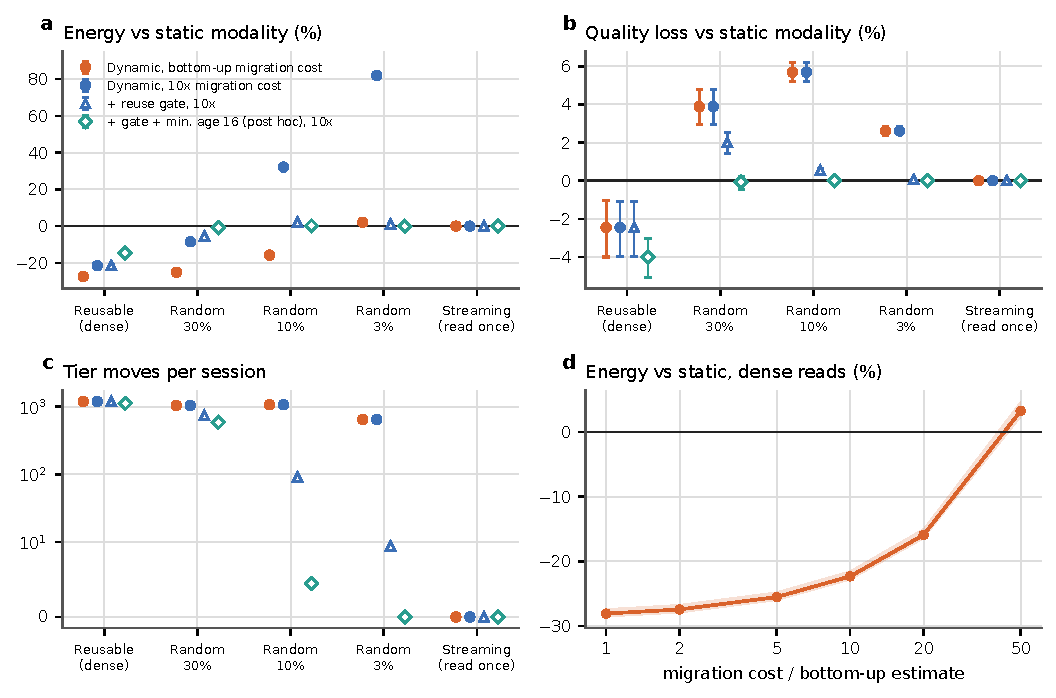
\includegraphics[width=\linewidth]{figs/fig_e9.pdf}
\caption{E9: (a) energy and (b) quality loss against static modality, by access regime (95\% CIs). (c) Tier moves per session. (d) Energy against migration cost in the dense regime (14 traces; band = 95\% CI): break-even near $45\times$ the bottom-up estimate. The green diamonds are the post-hoc variant.}
\label{fig:e9}
\end{figure}

\textbf{H9a, reusable data: confirmed.} Dynamic placement lowers energy by 27.4\% at the bottom-up cost (95\% CI $[26.9,27.8]$) and by 21.6\% at $10\times$ (E5's $-22.3\%$ in the first simulator), with quality 2.5\% better ($[1.1,4.0]$), 1190 moves per session, and a makespan penalty of 4.7\% and 13.1\% respectively.

\textbf{H9b, streaming data: confirmed, trivially.} With one read per entry, no entry is observed twice. The monitor's warm-up (Sec.~3.3) therefore never lets a move happen, and the dynamic and reuse-aware policies are identical to static modality in all metrics. The right decision for streamed data is simply the initial placement. The reason is worth stating because it is not a finding about the policy's cleverness: read-once data \emph{cannot repay} a migration, and the warm-up happens to encode that. (In this regime flat is 14\% \emph{faster} than static but uses $7.3\times$ the energy: the compute-site trade-off of E8 reappears with few reads.)

\textbf{H9c, random access: not confirmed as stated.} At $10\times$ migration cost the ungated dynamic policy is much worse than static when reads are sparse ($+32.1\%$ energy at 10\% reads, $+81.9\%$ at 3\%), because it pays $\sim$1000 moves per session for entries that are read too rarely to repay them. The gate removes most of the harm by suppressing 91\% and 98\% of those moves (1064$\to$91 and 645$\to$9) and brings the loss to $+2.2\%$ and $+1.1\%$, but our criterion was parity within 1\%, and the gate does \emph{not} meet it. With the bottom-up cost the break-even is only 1.08 reads, the gate never engages, and the dynamic policy saves energy under random access ($-15.8\%$ at 10\% reads, $-25.1\%$ at 30\%) \emph{but loses quality} ($+5.7\%$ and $+3.9\%$ against static; $+2.6\%$ at 3\%, where it also loses energy). Dynamic placement is therefore not regret-free under random access even when migration is cheap. Its thresholds were fitted to dense reads, and a monitor that only observes entries when they happen to be read is a plausible but untested cause.

\textbf{H9d, no single policy: half confirmed.} The best policy differs by regime: dynamic for reusable data, static for sparse random access (10\% and 3\%), either for streams. The second part (the reuse-aware policy never exceeds static by more than 2\% energy) fails narrowly: $+2.2\%$ at 10\% reads and $10\times$ cost.

\textbf{Post-hoc diagnosis of the residual (not part of the protocol).} After seeing H9c fail we asked why the gate still lets $\sim$90 moves through. A look at one trace (82 moves, 79 of them on prefill entries) suggested a noisy read-frequency estimate early in the session: an entry read a few times in its first steps looks highly reused. Requiring a minimum age before the estimate is trusted tests that explanation. With a minimum age of 16 steps the gate removes the residual at $10\times$: $+0.13\%$ energy ($[0.11,0.15]$) and neutral quality at 10\% reads, $0.0\%$ at 3\% (no moves), $-0.8\%$ at 30\%, with 4.5 moves per session at 10\%. The price is paid in the reusable regime, where delaying early moves cuts the saving from $-21.6\%$ to $-14.6\%$ (and $-27.4\%\to-20.0\%$ at the bottom-up cost). The choice matters: ages 4 and 8 leave $+2.15\%$ and $+1.06\%$. Because the variant was designed after seeing these test traces, with three ages tried, it is a diagnosis of where the regret comes from, not a tuned headline result.

\textbf{H9e, migration-cost sensitivity.} In the explicit model (dense reads, 14 traces, fixed thresholds) the saving is $-28.1\%$ at the bottom-up cost, $-25.5\%$ at $5\times$, $-22.3\%$ at $10\times$, $-15.9\%$ at $20\times$ and $+3.3\%$ at $50\times$ (CI $[+2.3,+4.7]$), a break-even near $45\times$ the bottom-up estimate, in agreement with E5's $\sim\!50\times$ from a different cost model. Migration traffic is 1\%, 8\%, 15\% and 31\% of total energy at $1\times$, $10\times$, $20\times$ and $50\times$, and the makespan penalty grows from $+4.6\%$ to $+47.6\%$: with a shared bus, migrations cost time as well as energy.

\begin{table}[t]
\centering\small
\caption{Pre-specified hypotheses of E8--E9 and their outcome.}
\label{tab:score}
\begin{tabular}{>{\raggedright\arraybackslash}p{1.0cm}>{\raggedright\arraybackslash}p{10.2cm}>{\raggedright\arraybackslash}p{3.8cm}}
\toprule
 & Statement (abbreviated) & Outcome\\
\midrule
H8a & Tiering moves $\ge$5$\times$ fewer bytes and uses $\ge$5$\times$ less energy than flat, at lower makespan & Confirmed ($11.8\times$, $9.3\times$, $0.64\times$)\\
H8b & Compute site matters: in-memory-only slower than flat at $\le$4 CIM units; adaptive within 10\% of the better pure strategy, cheaper than host-only & Confirmed (adaptive better than both)\\
H8c & Dynamic $\ge$10\% lower energy than static under contention, quality within $+2\%$ & Confirmed ($-27.4\%$, $-2.5\%$); $+4.7\%$ makespan\\
H9a & Reusable: dynamic $\ge$10\% lower energy, neutral quality & Confirmed ($-27.4\%$ / $-21.6\%$)\\
H9b & Streaming: dynamic $\approx$ static & Confirmed (identical; no moves)\\
H9c & Random, $10\times$ cost: ungated dynamic loses; gated within $+1\%$ of static & Ungated loses; \textbf{gate misses} ($+2.2\%$, $+1.1\%$)\\
H9d & Best policy differs by regime; gated never $>2\%$ worse than static & Half: differs; \textbf{misses} narrowly ($+2.2\%$)\\
H9e & Break-even migration cost (reported) & $\approx$45$\times$ the bottom-up estimate\\
\bottomrule
\end{tabular}
\end{table}

\textbf{What E8--E9 establish.} Computation placement is a first-order decision (a wrong default is $5\times$ slower than no tiering at 2 CIM units); a runtime that watches queue state beats both fixed choices on makespan; and whether dynamic \emph{data} placement pays depends on reuse: strongly for reusable data, not at all for streams, and under random access only if migrations are priced against the reuse the runtime has observed. The reuse-aware policy removes most but, as pre-specified, not all of the regret under random access.
